%; whizzy chapter
% -initex iniptex -latex platex -format platex -bibtex jbibtex -fmt fmt
% 以上 whizzytex を使用する場合の設定。

%     Tokyo Debian Meeting resources
%     Copyright (C) 2008 Junichi Uekawa

%     This program is free software; you can redistribute it and/or modify
%     it under the terms of the GNU General Public License as published by
%     the Free Software Foundation; either version 2 of the License, or
%     (at your option) any later version.

%     This program is distributed in the hope that it will be useful,
%     but WITHOUT ANY WARRANTY; without even the implied warranty of
%     MERCHANTABILITY or FITNESS FOR A PARTICULAR PURPOSE.  See the
%     GNU General Public License for more details.

%     You should have received a copy of the GNU General Public License
%     along with this program; if not, write to the Free Software
%     Foundation, Inc., 51 Franklin St, Fifth Floor, Boston, MA  02110-1301 USA

%  preview (shell-command (concat "evince " (replace-regexp-in-string "tex$" "pdf"(buffer-file-name)) "&"))
% 画像ファイルを処理するためにはebbを利用してboundingboxを作成。
%(shell-command "cd image200811; ebb *.jpg")

%%ここからヘッダ開始。

\documentclass[mingoth,a4paper]{jsarticle}
\usepackage{monthlyreport}

% 日付を定義する、毎月変わります。
\newcommand{\debmtgyear}{2008}
\newcommand{\debmtgmonth}{11}
\newcommand{\debmtgdate}{15}
\newcommand{\debmtgnumber}{46}

\begin{document}

\begin{titlepage}
\thispagestyle{empty}

% タイトルページ:編集必要な部分は最初のマクロに飛ばすこと

\vspace*{-2cm}
第\debmtgnumber{}回 東京エリア Debian 勉強会資料

\hspace*{-2.4cm}
\includegraphics[width=210mm]{image200801/2008title.eps}\\
\hfill{}\debmtgyear{}年\debmtgmonth{}月\debmtgdate{}日

\end{titlepage}

\dancersection{Introduction}{上川 純一}
 
 今月のDebian勉強会へようこそ。これからDebianの世界にあしを踏み入れると
 いう方も、すでにどっぷりとつかっているという方も、月に一回Debianについ
 て語りませんか?

 Debian勉強会の目的は下記です。

\begin{itemize}
 \item \underline{Debian Developer} (開発者)の育成。
 \item 日本語での「\underline{開発に関する情報}」を整理してまとめ、アップデートする。
 \item \underline{場}の提供。
 \begin{itemize}
  \item 普段ばらばらな場所にいる人々が face-to-face で出会える場を提供
	する。
  \item Debian のためになることを語る場を提供する。
  \item Debianについて語る場を提供する。
 \end{itemize}
\end{itemize}		

 Debianの勉強会ということで究極的には参加者全員がDebian Packageをがりがり
 と作るスーパーハッカーになった姿を妄想しています。情報の共有・活用を通し
 て Debianの今後の能動的な展開への土台として、「場」としての空間を提供す
 るのが目的です。

以上を目的とした、2008 年アジェンダです:
\begin{enumerate}
 \item 新年会「気合を入れる」
 \item Open Source Conference Tokyo (3/1)
 \item データだけのパッケージを作成してみる、
       ライセンスの考え方 (David Smith)
 \item バイナリ一つのパッケージを作成してみる (吉田@板橋)\\
       バージョン管理ツールを使いDebianパッケージを管理する(git)\\
       アップストリームの扱い(svn/git/cvs)(岩松 信洋さん)
 \item バイナリの分けたパッケージの作成。(前田さん)\\
       バイナリの分け方の考え方、アップグレードなどの運用とか。
 \item パッケージ作成(dpatch/debhelperで作成するパッケージ)(小林儀匡さん)\\
       man の書き方(roff or docbook)(でんさん)
       OSC 2008 Hokkaido
 \item パッケージ作成(kernel patch、kernel module)(岩松 信洋)
       Debconf発表練習(上川さん)

 \item Debconf アルゼンチン、共有ライブラリパッケージ作成
       コミックマーケット74

 \item Open Source Conference Tokyo/Fall、
       デーモン系のパッケージの作成、latex、 emacs-lisp、フォントパッケージ
 \item パッケージの cross-compile の方法、amd64 上で i386 のパッケージと
       か、OSC-Fall報告会、Debconf報告会
 \item 国際化 po-debconf / po化 / DDTP
 \item 忘年会
\end{enumerate}


\newpage

\begin{minipage}[b]{0.2\hsize}
 \definecolor{titleback}{gray}{0.9}
 \colorbox{titleback}{\rotatebox{90}{\fontsize{80}{80} {\gt デビアン勉強会} }}
\end{minipage}
\begin{minipage}[b]{0.8\hsize}
\hrule
\vspace{2mm}
\hrule
\tableofcontents
\vspace{2mm}
\hrule
\end{minipage}

\dancersection{事前課題}{岩松 信洋}


今回の勉強会の準備として、前日までに Debian GNU/Linux (sid) のインストールされたノートパソコンを用意していただき、
\LaTeX 環境を構築し、Debian 勉強会資料が作成できるまでを確認してもらいました。
これらの準備で発生した問題などを {\bf \LaTeX 合宿準備奮闘記}として提出していただきました。


\subsection{平澤}

centos5(utf-8)で \LaTeX をvimでつかっている平澤です。

Debianを触り始めたのがこの一年ぐらいから。
そもそもsidってなんだぁ?ってレベルで皆様にはご迷惑掛けてマス

今回のお題に触発されまして早速ノートPCのHDDをフォーマットして
クリーンインストール。

\subsubsection{Debian GNU/Linux sid のインストール}
 
debian sid のインストールは

\url{http://blog.wcrawl.com/archives/thinkpad_x41_debian_sid.html}

を参考にしてノートPCにsidをインストール。 
このページで'手間がかからない'方法をつかってみました。

この方法だと

\begin{commandline}
 hirasawa@debian-note:~$ cat /etc/apt/sources.list
 # deb http://ftp.jp.debian.org/debian/ sid main

 deb http://ftp.jp.debian.org/debian/ sid main
 deb-src http://ftp.jp.debian.org/debian/ sid main
 hirasawa@debian-note:~$ 
\end{commandline}

となる。
 
\subsubsection{パッケージのインストール}

下記の指定されたパッケージのうち
xpdf-japaneseとgs-cjk-resourcesをインストールするためには

\texttt{/etc/apt/sources.list}に \texttt{non-free}を追加する必要がありました。



\begin{commandline}
 # apt-get install \
 make ptex-bin dvipdfmx latex-beamer \
 okumura-clsfiles gs-esp xpdf xpdf-japanese whizzytex \
 evince \
 texlive-latex-extra \
 advi emacs22 yatex gs-cjk-resource gv git-core git-gui \
 qgit avahi-daemon \
 libnss-mdns avahi-autoipd 
\end{commandline}

\subsubsection{教材となる勉強会資料をチェックアウトしてビルド}

これ以降は指示の通りにやってみました。
(なにをやっているのかはわからない)

うちの非力PCだと20分以上やってますが.....(じつはまだ終わっていない)

流れている文字をみていると
なんかpdfがつくられているのが見える。(リアルタイムで中継中)
もうそろそろ終了か?

DellL400(Pen3 700MHzぐらい)で30分ぐらいかかって、debianmeetingresumeの
pdfがたくさんでてきました。

以上、debian初心者の平澤でした。

\subsection{あけどさん}

まずそもそもノートなマシンにDebianは入れていなかったので、空いてるノートを探したところ、Tadpole SPARCBook GS3
なんてのがあったのでそれにインストールを挑戦、結果は惨敗、敗因は実装メモリが
32MBというのが大きかったです。インストール要件には64MB以上となっていました・・・orz

仕方無いので、メインで使っている iBookG4(PPC)に環境を作成しました。
インストールに使ったCDはsarge用でAPT リポジトリの指定 (/etc/apt/sources.lst)
が何故かというかやはりというか stable (今だとetch)になってたのでちょっとハマったのはお約束?
他にも不要に見えたkernel-imageのパッケージを削除してboot出来なくなりインストールをやり直したりしました。orz
それ以外は、X-Windowも特にトラブル無くインストール出来、sarge → etch → sid と dist-upgrade
で楽に出来ました。XFree86からX.orgになったんだよなぁなどと感慨深いものがあったりしました。
何とか一応環境構築も出来まして上川さんの資料の PDF 生成までできました。

 ただ、そのままでは出来上がった PDF を表示しても日本語が空白になってしまいます。というか、そもそもデフォルトの GNOME 環境の
xpdf では日本語が表示できないようです。(何がまずいのかは未だ不明です。)

 なので、勉強会資料の PDF のプロパティを見てフォントが CMR10, CMSS17,・・・とあるので
\begin{commandline}
   # aptitude install cm-super cm-super-x11
\end{commandline}
としてフォントをインストールして
\begin{commandline}
   # aptitude install kpdf
\end{commandline}
で KDE 用 PDF ビューア をインストールする必要があるようです。
 他の PDF ビューア ePDFVewer でも日本語表示ができませんでしたのでその点は注意が必要かなと思います。

あと、山根さんご推薦のフォントを
\begin{commandline}
  # aptitude install ttf-kochi-gothic-naga10 ttf-kochi-mincho-naga10
\end{commandline}
としてインストールしました。

おまけ
iBookG4(PPC)へのインストールでは X-Window GDM で ']' キーが入力出来ない現象があり、キーマップを変更するのに
.xsession .initrc で xmodmap -e "keycode 51 = 0x5d" としても反映されませんでした。
これは{\bf .Xmodmap}に
\begin{commandline}
 keycode 51 = 0x005d 0x007d 0x005d 0x007d
\end{commandline}
と記載する必要がありました。
上記の各コードは normal shift かな かなshift の各入力モードにそれぞれ対応するようです。
なお、キーコードを調べるには Xterm などから
\begin{commandline}
 xev -display :0.0
\end{commandline}
としてテストウィンドウを開いて調べることが出来ます。
左Shift 右Shift もそれぞれキーコードが出力されるのでその点の留意が必要です。

\subsection{濱野さん}

ノートPC は会社から借りてるのしか持ってなくて普通に仕事で使っているので
sid にするのはカンベンしてください。
といっても、sid じゃないとダメな理由があるでしょうから、KVM/QEMU で仮想環
境を構築し、外付けUSBハードディスク内に sid の環境を用意してみました。

\begin{commandline}
 % dd if=/dev/zero of=vda.img seek=4G bs=1 count=0
 % mkdir ./mnt
 % mount -o loop vda.img ./mnt
 % debootstrap sid mnt/
 % echo "sid" > mnt/etc/hostname
 % echo "auto eth0" >> mnt/etc/network/interfaces
 % echo "iface eth0 inet dhcp" >> mnt/etc/network/interfaces
 % umount mnt/

 % qemu -m 256M -kernel vmlinuz-2.6.27.2 \
   -drive file=vda.img,if=virtio,boot=on \
   -append root=/dev/vda -k ja -curses -redir tcp:10022::22
\end{commandline}

sid の環境が出来ました。
ゲストにて
\begin{commandline}
 % apt-get make install ptex-bin dvipdfmx latex-beamer \
   okumura-clsfiles gs-esp xpdf xpdf-japanese whizzytex evince \
   texlive-latex-extra advi emacs22 yatex gs-cjk-resource gv \
   git-core git-gui qgit avahi-daemon libnss-mdns avahi-autoipd
\end{commandline}

いろいろ入りました。
ゲストのカーネルを削ってしまったせいか、途中 CONFIG\_HIBERNATION=y にしろ
とか言われましたが無視しました。
\begin{commandline}
 % git clone git://git.debian.org/git/tokyodebian/monthly-report.git
 % cd monthly-report
 % cp -p git-pre-commit.sh .git/hooks/pre-commit
 % time make
 % ls *.pdf
\end{commandline}

10 分程度で PDF が出来上がりました。
ゲスト側に windomanager などが入っていないので、ホスト側に持ってきて
xpdf で読んでみるとばっちり日本語も表示されました。
当日までにゲスト側の X の環境も整えておこうとおもいます。

また、texlive を使うのは初めてなのでのでハンズオンを楽しみにしています。

\subsection{前田さん}
普段からSidの環境を使っているので、環境の準備という点では特に困ったことはありませんでした。
以前、MacBook Airを64bit化したときにはちょっと苦労したことはありました\footnote{\url{http://d.hatena.ne.jp/mkouhei/20080713\#1215913997}}が、
今回の課題とは論点が外れるので省略。
\LaTeX の環境も、5月度の勉強会のときに環境を整備していたので、こちらも特に苦労せず。
あえて言えば、gitを普段から使っていないので、以前git cloneで取得したDebian勉強会のリポジトリを
最新状態に更新する方法と、yatexの設定を.emacsのどこに書くのかを調べました。

気になったのはPDFが110くらいではなく、95しかできていないのは何故か?
何か足りないものがあるのでしょうか。(あまり追求せず)

細かく挙げると意外とあるもんですね。


\subsection{山本さん}
{\bf 奮闘}と言うほど、奮闘はしていません。

\begin{enumerate}
\item Debian GNU/Linux sid のインストール
Note PC は元々 sid をインストールして使ってました。

\item パッケージのインストール
aptitude を使いインストール。Recommends は入れてません。

\item 教材となる勉強会資料をチェックアウトしてビルド
パッケージを入れた時 (3 週ぐらい前の時点) では何の問題もなくビルドできました。
勉強会直前にまたチェックアウトして試してみます。
\end{enumerate}

\subsection{やまださん}
今回はじめてDebian勉強会に参加させていただきます、やまだです。
事前にノートPCにsidと \LaTeX の環境を準備することになっていましたので、その状況を説明します。

ハードウェア: Sony VGN-Z70B (\url{http://www.vaio.sony.co.jp/Products/Z1/})

インストール方法: Windows Vista上のVMwareにDebian環境を構築する

\begin{enumerate}
\item Windows Vista上に、フリーのVMware Serverをインストールしました\\
VMware Serverの利用は初めてだったのですが、セキュリティ証明書に問題がある点を除けば比較的スムーズにインストールできました。

\item VMware ServerにDebianをインストールしました\\
sidのインストールは初めてだったのですが、先にdebian-users
MLに情報が流れてしまいましたので、比較的スムーズにインストールできました。 (See [debian-users:51105] )
次のWebページを参考にしました。 \url{http://blog.wcrawl.com/archives/thinkpad_x41_debian_sid.html}

\item パッケージをインストールしました\\
/etc/apt/sources.list に non-free を追加する必要がありましたが、debian-users ML
の情報があったのですぐ解決できました。

\item 教材となる勉強会資料をチェックアウトしてビルドしました\\
ビルドは問題なく完了しました。
\end{enumerate}
\TeX は大昔に本を読んだり軽く触った程度の経験しかなく、本格的に \LaTeX を使ったことはないので、今回の勉強会で勉強させていただきます。


\subsection{Motohara さん}
Debian勉強会には初めて参加させて貰いますmatoharaといいます。
Debian はServer 用途に使うことが多いです。

事前準備の報告です。
Etch で利用しているNotePC をsourcer.list を書き換えてsid にdist-upgrade
しました。
パッケージの導入でつまずきましたがsource.list にnon-free を登録すること
で回避できました。

この後、データの取得まではよかったのですが約90分とmake にとても時間が掛
かってしまいました。
このマシンのCPU はAMD GeodeLX 500Mhz なのでこれが利いているのだと思います。

これでは当日も辛そうなのでMacBook(Core2Duo 1.8MHz) に仮想マシン
(ParallelsDesktop4.0)としてsid を導入してみたところ9分ほどでmake 終了し
ました。
当日はこちらのマシンで参加しようと思います。
ちなみに今回初めて不安定版の新規インストールの方法を知りました。

\LaTeX はほぼ初めてなので少し不安ですがよろしくお願いします。

\subsection{きたはらさん}
デスクトップも {\bf Etch} を常用しているので、
{\bf sid}のインストールが初体験で、その方法を調べる
所から結構悩みました。
git関係も以前の勉強会で学習していたはずですが、
すっかり忘れていて、以前の資料を引っ張り出したり
して苦労しました。
最終的にpdfは出来たのですが、上記で作成した
{\bf sid}環境で日本語フォントの部分が表示されず、
いまだ未解決。 勉強会に間に合うか?
(当該ファイルも、某OSでは問題なく表示でき、日本語
フォントが埋め込まれている資料は、問題なく表示出来
るので、ドキュメントビューアの代替フォントの設定の
問題なのかと思っているのですが…)

\subsection{鈴木さん}
sid環境作成するのが大変でした。まずなによりも不覚だったのは、stableを間違ってインストールし終わってから課題メールを読みはじめたこと。
この時点で締切り残り1時間強。
sidインストールは特に問題なかったです。ダウンロード時間以外は。そしてここでタイムオーバーの11/13の24時を迎えてしまいました。
pdfのほうも問題なくできあがりましたが、debianで日本語が見られる環境になっていなく、他の環境で確認しました。
勉強会までに見られるようにしておきます。

\subsection{じつかたさん}
元々、MacBookのVMware上にsidがインストール してあったので、パッケージのみインストールしました。
pdfの生成も完了しました。sidがインストール済みでしたの で、比較的楽でした。
ただ、\LaTeX をまったく使ったことがないので、事前に勉強し ていこうと思っています。
が、これ(事前課題)を提出する時点で、まったく勉強 ができていません。

\subsection{藤沢さん}
 既に期限を過ぎてしまっていますが、提出します。
 Debian sidが必要ということで、まずはsidのインストールからはじめました。sid
は今まで自力でインストールしたことがなかったのですが、ここでいきなりつまづい
てしまいました。
 ノートPCということでMacBookに入れようとしたのですが、インストールしてみる
と、X Windowがなにやらエラーをはいて、そのまま真っ黒に……。そもそも作業を始
めたのが遅かったので、6時間くらいで断念しました。
(エラーの内容を記録し忘れました……。無念)
 その後、別のノートPCを用意してVMWare上で動かすことにし、こちらもインストー
ル。こちらは上手くいきました。その後の各種設定は大きな問題もなくスムーズにで
きたので、奮闘したのはインストール作業のみです。
 MacBookで動かせなかった問題は、近いうちに解決してやろうと心に誓いました。

\subsection{伊藤さん}
 既に期限を過ぎてしまっていて大変もうしわけないです。

特に苦労したという訳でも無いですが、evinceの日本語フォントの設定が入っておらず
日本語のPDFを表示できずに気まずい状態だったので以下の様にフォントのシンボリックリンクを作ってあげました。
\begin{commandline}
$ sudo apt-get install cmap-adobe-japan1
$ sudo ln -s /usr/share/xpdf/japanese/Adobe-Japan1.cidToUnicode
/usr/share/poppler/cidToUnicode/Adobe-Japan1
$ sudo mkdir -p /usr/share/poppler/cMap
$ sudo ln -s /usr/share/fonts/cmap/adobe-japan1
/usr/share/poppler/cMap/Adobe-Japan1
$ evince debianmeetingresume200502.pdf
\end{commandline}
こういう場合の対応のフィードバックをどうすればいいかを学んでフィードバック出来るようになるのが
自分の課題だなと思っております。


\subsection{岩松信洋さん}
普段から sid を使っているのと、\LaTeX で資料を作成しているので、特に問題はありませんでした。
普段の書き方としては、Emacs をメインで使っていないため、細かい使い方が分からず、Emacs で編集、
コンパイル後、evince でリロードで確認という方法をとっています。
今回、ちょっと大人になってみるか、ということで上川さんがおすすめする whizzytex をインストールして
使って見ました。大きな画面では使いやすいですが、ノートパソコンではちと使いづらいという印象です。
また、whizzytex は vim などで使えないようなので、メンテナである上川さんに vim でも使えるように
していただきたいと思います。

\subsection{森田尚さん}


LaTeX合宿準備奮闘記

パッケージのインストールと勉強会資料のビルドは問題なくできました。
WhizzyTeXがうまく動きませんが、当日までになんとかするつもりです。

\LaTeX{}は仕事でも使っていますが、いまだに得意ではありません。
以下思いついたところを書き並べてみます。

LaTeX関係で作って公開しているもの:
\begin{itemize}
 
 \item  multipagebox.sty
	\footnote{\url{http://hisashim.livejournal.com/398344.html}}\\
    ページをまたげる囲み罫のパッケージです。
    
 \item  vfdata-otf-ptex
	\footnote{\url{http://sourceforge.net/projects/ideotype}}\\
	OpenTypeを扱うためのOTFパッケージのDebianパッケージです。
\end{itemize}

LaTeXについて知りたいこと:

\begin{itemize}
 \item  次世代日本語TeXの動向(特にUnicodeサポート)
	\begin{itemize}
	 \item  epTeX, upTeX, eupTeX
	 \item  ptexlive
	\end{itemize}    
いずれも香田さんがDebianパッケージ化作業中?

 \item  マクロをテストする方法\\
    traceで追いかけるのに疲れたのでtexunit.styを書きかけましたが
    挫折しました。良い方法があれば教えてください。
\end{itemize}

LaTeXと関係ないけれど知りたいこと:

\begin{itemize}
 \item tex4htをpTeXで使う方法
\end{itemize}


\subsection{日比野 啓}

当日に提出して大変申し訳ないです。
当然のように載ってないのでここに書いてみます。

普段使っている{ \bf Think pad } に自分の環境を壊さないように設定を追加していってみました。
今回追加するパッケージのうち、もともと入っていなかったのは、
dvipdfmx latex-beamer okumura-clsfiles texlive-latex-extra whizzytex advi yatex
git-gui qgit avahi-daemon avahi-autoipd libnss-mdns
でした。
avahi関係以外はサクっとインストールしました。
avahi関係は普段使っていないのと、ネットワークが使えなくなってハマったことがあったので、
パッケージのダウンロードだけしてきました。
gitでのmonthly-reportのcheckoutからpdfのbuildも問題なく終わりました。

あんまり関係ないですが、a4j + jsarticleだとdvipdfmxがうまく動かない問題があるようです。
\begin{verbatim}
>** WARNING ** Could not open config file "fontmapsx".
\end{verbatim}
みたいなエラーが出ます。

\begin{verbatim}
\documentclass[a4j]{jsarticle}
\begin{document}
ほげほげ
\end{document}
\end{verbatim}
みたいな.texで.dviを出力してちょっと strace -f dvipdfmx hogehoge.pdf してみると

\begin{verbatim}
>stat("/etc/texmf/dvipdfm/fontmapsx", {st_mode=S_IFREG|0644, st_size=60, ...}) = 0
>...
>access("./fontmapsx", R_OK)             = -1 ENOENT (No such file or directory)
>...
>write(2, "Could not open config file \"fontm"..., 39Could not open config file "fontmapsx".) = 39
\end{verbatim}

変な場所にfontmapsxを探しにいくようです。
kpathsearchの問題? でしょうか。


%%% trivia quiz
\dancersection{Debian Trivia Quiz}{岩松 信洋}

ところで、みなさん Debian 関連の話題においついていますか?Debian関連の話
題はメーリングリストをよんでいると追跡できます。ただよんでいるだけではは
りあいがないので、理解度のテストをします。特に一人だけでは意味がわからな
いところもあるかも知れません。みんなで一緒に読んでみましょう。

今回の出題範囲は\url{debian-devel-announce@lists.debian.org} に投稿された
内容とDebian Project Newsからです。

\begin{multicols}{2}
 \subsection{debian-devel-announce}
 \url{debian-devel-announce@lists.debian.org}への投稿内容からです。

 \santaku
 {BTS 500000番はどんなバグ報告だったでしょうか}
 {SPAMだった}
 {cdbs に defoma 対応させるためのパッチ}
 {Lenny リリースが遅れているというバグ報告}
 {B}
{}

 \santaku
 {10月25日から30日まで行われた BTS の景品は何でしょう?}
 {DPLからのキス}
 {次回のDebconf無料チケット}
 {おいしいクッキー}
 {C}
{}
 
 \santaku
 {screenshots.debian.net は何をまとめたサイトでしょうか?}
 {デスクトップのスクリーンショット}
 {ソフトウェアのスクリーンショット}
 {Debian Developerのプライベート写真集}
 {B}
{}

 \santaku
 {Joerg Jaspertがプロポーザルを出したDebian membershipとは?}
 {「Debian開発者」の現在の定義を変えるための提案}
 {Debian開発者の家族に関する提案}
 {Debianからforkしたディストリに関する提案}
 {A}
{}
 % http://lists.debian.org/debian-devel-announce/2008/10/msg00005.html

 \santaku
 {Debian Installer team から出たアナウンスは何でしょう?}
 {ごっめーん!インストーラー遅れちゃった。}
 {Debian Installer lenny RC1 出たよ}
 {RC1 は飛ばして リリースする予定です。}
 {A}
{}
\end{multicols}
 
\dancersection{最近のDebian関連のミーティング報告}{岩松 信洋}
\subsection{東京エリアDebian勉強会45回目報告}
東京エリアDebian勉強会報告。 10月の第45回東京エリアDebian勉強会を実施しました。
今回のDebian勉強会は、OSC 2008 Tokyo/Fallで行い、参加者は、やまねさん、前田さん、明渡さん、斉藤さん、日比野さん、山本さん、小室さん、本上さん、たかすぎさん、小林さん、岩松の11名でした。
セミナーとして、やまねさんが 「あなた」とオープンソース/フリーソフトウェア、そして「Debian」という題名で、岩松が、オープンソースでの Flash 再生環境という題名でお話させていただきました。
やまねさんのセミナーは大盛況でしたが、岩松のセミナーは人がいませんでした。内容がマニアックすぎるのと、朝一のセミナーだっただめと思っておきます。
また、勉強会大集合 として、東京エリアDebian勉強会の紹介を岩松がお話させていただき、勉強会に関して、パネルディスカッションを行いました。
このパネルディスカッションでは、各勉強会の運営方法やメリットデメリットについて話しました。今後、いろんな勉強会が増えるといいですね。

ブースでは、eeepc on Debian , USB顕微鏡、PPC, ARM マシンの展示、過去の資料の展示、LennyインストールDVDの配布意を行いました。
いろんな方がブースに寄られ、さまざまな意見交換が行われたようです。
OSCが終わった後、Ubuntu関係の方と割烹 二葉 で宴会をしました。


% (query-replace-regexp "<.*?>" "")
% (query-replace-regexp "^[	 ]\+" "")

\dancersection{Debconf8 参加報告}{上川 純一}
\label{sec:debconf8}
\index{debconf8}
\index{Debian Conference 2008}

\subsection{Debconfとは}

  2008年度の Debconf は 8月10日から8月16日まで、アルゼンチンのマルデル
プラタで行われました。日本からは、上川 純一が参加しました。

\subsubsection{Debconfの歴史・経緯}

Debian Conference \url{http://debconf8.debconf.org/} は Debian 
の開発者たちが一同に介するイベントです。通常顔をあわせることのないメンバー
たちが一同に介し友好を深め、技術的な議論を戦わせます。過去の開催履歴を見
てみると\tbref{tab:debconflist8}のようになります。

\begin{table}[H]
\caption{歴代のDebconf参加者推移}
\label{tab:debconflist8}
 \begin{center}
 {\footnotesize
 \begin{tabular}{|c|c|c|r|}
 \hline
 年 & 名前 & 場所 & 参加人数 \\
 \hline
 2000 & debconf 0 &フランス ボルドー & \\
 2001 & debconf 1 &フランス ボルドー & \\
 2002 & debconf 2 &カナダ トロント & 90名 \\
 2003 & debconf 3 &ノルウェー オスロ & 140名 \\
 2004 & debconf 4 &ブラジル ポルトアレグレ &  150名 \\
 2005 & debconf 5 &フィンランド ヘルシンキ & 200名 \\
 2006 & debconf 6 &メキシコ オアスタペック & 300名 \\
 2007 & debconf 7 &英国スコットランド エジンバラ & 約400名 \\
 2008 & debconf 8 &アルゼンチン マルデルプラタ & 約200名 \\
 \hline
 \end{tabular}
 }
 \end{center}
\end{table}

\subsubsection{Debconf 2007} 2008年度の Debconf は海辺のホテルを二棟借
りて開催しました。宿泊しているホテルの7Fと1Fがハックラボになっており、
7Fがカンファレンスルームになっているという便利な環境でした。

\subsection{アルゼンチン・マルデルプラタ}

\subsubsection{行き方}
  日本からアルゼンチンまでは、直行便がありません。
  上川はサンフランシスコ・カナダのトロント・チリのサンチャゴを経由して
  アルゼンチンのブエノスアイレスまで移動(ここまでで約30時間程度)、
  そこからバスで移動(5時間(直行)から10時間(乗り換え))しました。

  今回の会期は従来と違い長期休暇でバカンスをとっている人の多い時期です。
そのため、飛行機の予約のタイミングが難しかったかもしれません。
また、日本からアルゼンチンにいく便には安いものがあまりみつからず苦労しました。

ブエノスアイレスからマルデルプラタの間は東京・大阪間程度の距離があり、
多数のバスが通っています。空港からブエノスアイレスの市街で乗り換えれば多数のバスがあるのですが、
空港からの直行のバスは非常に少なく(Manuel Tenda Leonという会社のバスのみが運行している模様)、
予約ができない人がでていたようです。

\subsubsection{会場}

\begin{wrapfigure}{r}{6cm}
  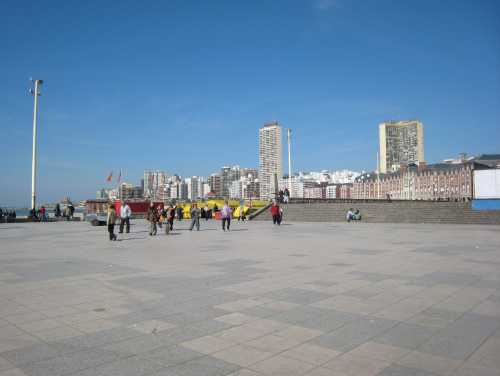
\includegraphics[width=\hsize]{image200810/mdq-area.jpg}
\end{wrapfigure}
会場はビーチリゾートとして知られるマルデルプラタの中央カジノ前のホテルでした。
\\


\subsection{スケジュール}

8月10日から開始し、8月16日までイベントがぎっしりつまっていました。
8月18日にブエノスアイレスに移動し、そこでDebian Day を開催しました。

\subsection{会期中で気になったこと}

上川が今回参加して気になったことを紹介します。

Debconf に参加しているミラーサーバはフルミラーではなくアーキテクチャ
i386, amd64, ppc と armel でした。

qemubuilder を開発している関係でarmel関連の作業を行いました。
qemubuilder の armel 移植と、armel 関連のデバッグなどです。
しかしながら途中でPCのHDDが故障し後半はHDDの購入からインストール、
macbookのブートローダのデバッグに費しました。

PGPキーをICカードで利用する仕組みがあるみたいで、作成していました。
ただ、仕組みがよくわからないので今回はスルーしました。

%
\dancersection{「その場で勉強会資料を作成しちゃえ」 Debian を使った \LaTeX 原稿作成合宿}{上川 純一}
\label{sec:latexdebmtgres}
\index{latex}

\subsection{概要}

Debian 勉強会では資料を \LaTeX で管理しています。
Emacs, Git, \LaTeX で Debian 勉強会資料作成をする流れを体験してみましょう。

ハンズオンでDebian 勉強会資料のチェックアウト、作成からコミットまでの流れ
を一通り試します。途中でつまったらできるまで現地で対応する予定です。
\footnote{ベストエフォート、もしかするとできない場合もあります}。

\subsection{事前準備}

当日の時間は限られているため、事前準備が必要です。
現地に入るまでに準備しておくものです

\begin{itemize}
 \item 無線LAN接続可能なノートパソコン
       (十分長いLANケーブルを持参しても可能、スイッチも持参してください)
 \item 必要なパッケージをインストールした Debian GNU/Linux sid のシステ
       ム
 \item 記事にする内容。
       紹介したいツール/パッケージ関連のコマンドライン出力と
       画面写真と簡単な説明文章。
\end{itemize}

事前にインストールしておいて欲しい必要なパッケージは

\begin{itemize}
 \item 基本ツール: make 
 \item \LaTeX 一式: ptex-bin dvipdfmx latex-beamer  okumura-clsfiles
       ghostscript-x\footnote{lenny以前での gs-esp 相当} xpdf 
       xpdf-japanese evince poppler-data texlive-latex-extra
 \item emacs / whizzytex 関連一式: whizzytex advi
       emacs22-gtk\footnote{emacs22 でもよい、emacs22-nox は難しいかも} 
       yatex gs-cjk-resource gv
 \item Git 関連一式: git-core git-gui qgit
 \item DHCP / Avahi 関連一式: avahi-daemon avahi-autoipd libnss-mdns
 \item 日本語フォント関連: ttf-mona ttf-sazanami-mincho ttf-vlgothic
 \item 日本語入力関連: scim-anthy 
 \item 日本語必須ツール: lv\footnote{lgrepなど}
\end{itemize}

avahi の設定が正しいことは、ping ホスト名.local が使えるかどうかで確認し
ます。/etc/nsswitch.conf の hosts 行にmdns\footnote{なんらかの mdns の設
定であればよく、例えば mdns4 であってもよい。}を参照する設定が追加されている
ことを確認してください。

\begin{commandline}
hosts:          files mdns dns
\end{commandline}

% 実験的には念のため apt-get には -o APT::Install-Recommends=false を指定
% して確認している。 

\begin{commandline}
# apt-get update
# apt-get install \
 make ptex-bin dvipdfmx latex-beamer \
 okumura-clsfiles ghostscript-x xpdf xpdf-japanese whizzytex \
 evince poppler-data \
 texlive-latex-extra \
 advi emacs22-gtk yatex gs-cjk-resource gv git-core git-gui \
 qgit avahi-daemon \
 libnss-mdns avahi-autoipd \
 ttf-mona ttf-sazanami-mincho ttf-vlgothic \
 scim-anthy
# jisftconfig add
\end{commandline}
\footnote{okumura-clsfiles の依存する ptex-jisfonts はインストール後に手
動で設定をする必要がある。
具体的には jisftconfig add を実行。}

事前にダウンロードしてビルドできる環境であることを確認しておいてください。

\begin{commandline}
$ git clone git://git.debian.org/git/tokyodebian/monthly-report.git
$ cd monthly-report
$ cp -p git-pre-commit.sh .git/hooks/pre-commit
$ make -j4 
$ ls *.pdf # 110くらいのPDFファイルが生成されていることを確認
\end{commandline}

Emacs の設定をします。
yatex の設定と
文字コードの設定をします。

.emacs に

\begin{commandline}
;; YaTeX が漢字コードを毎回ISO-2022-JPに設定しないようにする
(setq YaTeX-kanji-code nil)

;; git.el をロードする
(load-library "/usr/share/doc/git-core/contrib/emacs/git.el")
\end{commandline}

Git の設定もしておきましょう。
ユーザ名とメールアドレスを設定します。
設定しないとホスト名や /etc/passwd の設定をデフォルトで使ってしまいます。

\begin{commandline}
$ git config --global user.email dancer@netfort.gr.jp
$ git config --global user.name "Junichi Uekawa"
\end{commandline}

\subsection{演習0: 環境設定}

勉強会の会場で準備している環境です

\begin{itemize}
 \item avahi 経由で接続できる Debian package cache (i386, amd64)
 \item 無線LAN(WEP) ESSID:XXXXX 
\end{itemize}

DHCPでネットワーク接続してください。
avahi(mDNS) で名前解決できることを確認してください。
apt リポジトリの設定が可能であることを確認してください。


\begin{commandline}
# ping coreduo.local
# cat /etc/apt/sources.list
deb http://coreduo.local:9999/debian/ sid main contrib non-free
# apt-get update 
\end{commandline}


\subsection{演習1: リポジトリチェックアウト}

\begin{commandline}
$ git clone git://coreduo.local/git/monthly-report.git
\end{commandline}

\begin{commandline}
$ make -j4 # エラーがでます
$ cp -p git-pre-commit.sh .git/hooks/pre-commit
$ make -j4
\end{commandline}


\subsection{演習2: emacs whizzytex 起動}

\begin{commandline}
$ cd XXXXX
$ emacs
\end{commandline}

whizzytexを起動します。
プリビューが開始するというメリットだけでなく、即時コンパイルエラーを検出
できるのが重要です。

\begin{commandline}
M-x whizzytex-mode 
\end{commandline}

スペルチェックも起動しましょう。\footnote{iamerican もしくは ibritish パッ
ケージが必要です。}

\begin{commandline}
M-x flyspell-mode
\end{commandline}

\subsection{演習3: セクションを追加}

まずセクションを追加します。

\begin{commandline}
\dancersection{XXXX}{名前}
\index{XXXX@YYYY}
\label{XXXX@YYYY}

% 本文

\end{commandline}

\subsection{演習4: 説明の章だてを書いてみる}

\begin{commandline}

\subsection{xxxx}

\subsection{xxxx}

\subsection{xxxx}

\subsection{xxxx}

\subsection{xxxx}

\end{commandline}

\subsection{演習5: 説明の中身を書いてみる}

文章は空行区切りでパラグラフになります。roffなどと同じです。
改行は無視されます。

\verb!\!ではじまる文字列が命令です
\begin{commandline}
 \XXXX{YYYY}
\end{commandline}

monthlyreport.sty で追加のコマンドが定義されています。
\footnote{フットノートが追加できます}

表を作ってみましょう。

\begin{table}[h]
\caption{キャプション}
\label{tab:1234}

 \begin{tabular}{|c|c|c|}
 \hline
 ディストリビューション & バージョン & 備考 \\
 \hline
 ディストリビューション & バージョン & 備考 \\
 ディストリビューション & バージョン & 備考 \\
 \hline
 \end{tabular}
\end{table}


知っておきたい構文は実はあまりたくさんはありません。
利用されている上位:

\begin{commandline}
$ sed -n 's/.*\(\\[a-z]\+\).*/\1/pg' *.tex  | sort | uniq -c | sort -rn  
   6948 \item
   6240 \end
   5628 \begin
   1952 \subsection
   1623 \subsubsection
   1491 \santaku
   1258 \url
   1189 \hsize
    895 \hline
    874 \texttt
    522 \dancersection
    473 \footnote
    451 \includegraphics
    447 \vspace
    405 \label
    378 \frametitle
    357 \usepackage
    323 \hspace
    316 \hrule
    300 \section
    253 \bf
    236 \index
\end{commandline}

利用されている上位の begin-end 構文

\begin{commandline}
$ sed -n 's/.*\(\\begin{[a-z]\+\).*/\1/pg' *.tex  | sort | uniq -c | sort -rn 
   1742 \begin{itemize
   1293 \begin{commandline
   1245 \begin{frame
    781 \begin{minipage
    271 \begin{center
    194 \begin{enumerate
    148 \begin{tabular
    133 \begin{figure
\end{commandline}

\newcommand{\debiangnulinux}{Debian GNU/Linux}

\debiangnulinux{}のようによく使う文字列はnewcommandで定義できます。
ただし、命令がファイル毎に別の意味を持つようになると
管理がしにくくなるのでできるだけ monthlyreport.sty に定義は集中させています。
monthlyreport.sty は共有しているので変更する際には御注意を。最初は変更内容につ
いて誰かにレビューをお願いしたほうがよいと思います。

\begin{commandline}
$ git log --pretty=format:%an monthlyreport.sty | sort | uniq -c 
     15 Junichi Uekawa
      3 Nobuhiro Iwamatsu
\end{commandline}

エスケープが必要な文字列の出力方法
\begin{itemize}
 \item \verb!\! verb は見にくくなるので最終的手段
 \item \~{}
 \item \^{}
 \item aaaa$<$aaaa そのままだと:<
 \item aaaa$>$aaaa そのままだと:>
 \item aaaa\#aaaa
 \item aaaa\%aaaa
 \item \_{}aaaa
\end{itemize}

よく使うコマンド
\begin{itemize}
 \item begin itemize / item / end itemize
 \item begin enumerate / item / end enumerate
 \item commandline (勉強会用に定義)
 \item includegraphics 後述
 \item 
\end{itemize}

\subsection{演習6: コマンドライン出力を追加してみる}

\begin{commandline}
\ begin{commandline}

コマンドライン出力

\ end{commandline}
\end{commandline}

\subsection{演習7: png 画像を挿入してみる}

includegraphics

png 

git add

ebb

make で確認。

\subsection{演習8: git で変更をコミットしてみる}

\begin{commandline}
$ make 
\end{commandline}

\begin{commandline}
M-x git-status
\end{commandline}

\subsection{演習9: git での変更を送信してみる}

\begin{commandline}
$ git pull
\end{commandline}

コンフリクトを解消します。

\begin{commandline}
M-x git-status
\end{commandline}

\begin{commandline}
$ git push
\end{commandline}

\begin{commandline}
$ mkdir ~/patches/
$ git format-patch -o ~/patches/ HEAD^ 
\end{commandline}
生成されたパッチファイルをメールで送付します。

\subsection{演習10: git で変更をマージしてみる}

\subsection{演習11: 全体を眺める}

outline-minor-mode が便利です。


\subsection{今回演習できないTIPS}

\subsubsection{alioth tips}
資料の編集には alioth を利用します。
alioth.debian.org, git.debian.org です。

アカウントを作成します。
Debian Developer でないばあい、
XXXX-guestというユーザ名になります。

便利につかうため、\texttt{.ssh/config} に設定を追加しましょう。

\begin{commandline}
ServerAliveInterval 10
ServerAliveCountMax 12

Host alioth.debian.org
 ControlMaster auto
 ControlPath ~/tmp/ssh-%r@%h:%p
 User xxxx-guest

Host git.debian.org
 ControlMaster auto
 ControlPath ~/tmp/ssh-%r@%h:%p
 User xxxx-guest

Host localhost
 StrictHostKeyChecking no

Host *.local
  CheckHostIP no
\end{commandline}

%\printindex

\cleartooddpage

\vspace*{15cm}
\hrule
\vspace{2mm}

\includegraphics[width=2cm]{image200502/openlogo-nd.eps}
\noindent \Large \bf Debian 勉強会資料\\ \\
\noindent \normalfont \debmtgyear{}年\debmtgmonth{}月\debmtgdate{}日 \hspace{5mm}  初版第1刷発行\\
\noindent \normalfont 東京エリア Debian 勉強会 (編集・印刷・発行)\\
\hrule


\end{document}
